\documentclass[13pt, a4paper, twoside]{article}
\usepackage[utf8]{inputenc}
\usepackage{geometry}
\usepackage[czech]{babel}
\usepackage{chemformula}
\usepackage{chemfig}
\usepackage{enumitem}
\usepackage{float}
\usepackage{fancyhdr}
\usepackage{caption}
\usepackage{setspace}
\usepackage{multicol}
\geometry{legalpaper, margin=1.05in}
\pagestyle{fancy}
\lhead{\Large Šárka Doležalová, skupina 6}
\rhead{\large 10.12.2020}
\begin{document}
\begin{center}
    \Huge
    Úloha 10: Stanovení rozpustnosti a obsahu krystalové vody
\end{center}
\large \onehalfspacing
\section*{Zadané úlohy}
\begin{enumerate}
    \item Stanovte rozpustnost předloženého vzorku anorganické soli ve vodě při laboratorní teplotě.
    \item Na základě naměřených údajů identifikujte neznámý vzorek.
    \item Termogravimetricky stanovte množství krystalové vody v předloženém vzorku.
\end{enumerate}

\section*{Teoretický úvod}
\subsection*{Rozpustnost látek}
Gibbsův zákon fází popisuje rovnováhu v uzavřeném systému rovnicí: $f+v = s +2 $.
ve které je f počet fází, v počet stupňů volnosti a s počet složek v systému. Fáze jsou homogenní složky (plyn, kapalina, pevná fáze) systému a složky jsou jednotlivé chemické sloučeniny. Stupeň volnosti je jakákoliv intenzivní fyzikální veličina. Intenzivní veličina je taková, která nezávisí na celkové hmotě systému.

\subsection*{Krystalová voda}
Když látky krystalizují z vodném prostředí do sebe často zabudovávají molekuly vody do struktury krystalu. Krystalové vody se může snadno zbavit stáním krystalických vzorků na vzduchu.

\subsection*{Práce s automatickou pipetou}
Automatická pipeta se používá o odměření velmi malých objemů. Daný objem se nastavuje šroubem v horní části pipety. Pipetu nesmíme nikdy obracet napo pokládat na stranu, pokud je na ní nasazena znečištěná špička.

\subsection*{Zahřívání nad kahanem a žíhání do konstantní hmotnosti}
Žíhání je specifickým laboratorním postupem provádějícím se nad kahanem, obvykle v porcelánových miskách. Kelímek je zahříván pomalu, aby nepraskl, poté je přesunut do nejteplejší části plamene. K žíhání můžeme také používat žíhací pec.
Žíhání do konstantní hmotnosti můžeme využít například při gravimetrii. 

\section*{Postup}
\subsection*{Stanovení rozpustnosti a identifikace vzorku}
Nad kahanem byly vyžíhány tři kelímky do konstantní hmotnosti. Žíhání probíhalo cca 10 minut a kelímky byly pomocí kleští přesunuty do exsikátoru k vychladnutí. Vychladlé kelímky byly zváženy na analytických vahách. Žíhání kelímků bylo zopakováno. Kelímky byly znovu zváženy a hmotnosti byly porovnány. Kdyby se hmotnosti měnili, proces by byl zopakován. Byla změřena teplota suspenze neznámého vzorku (č.105), poté co byl vzorek rozmíchán a bylo počkáno 5 minut. Do vyžíhaných kelímků bylo pomocí automatické pipety odpipetováno 5 ml nasyceného roztoku a byla zapsána hmotnost roztoku. Voda z odpipetovaných roztoků byla opatrně odpařena. Po odpaření vody, byl zbytek v kelímcích žíhán ještě dalších 10 minut. Po vychladnutí v exsikátoru byly kelímky zváženy a kelímky byly žíhány do konstantní hmotnosti.

\subsection*{Plamenová zkouška}
Předem vyžíhaný drátek byl ponořen do neznámého vzorku a poté byl vložen do plamene. Podle jeho barvy byl určen kationt v roztoku.

\subsection*{Stanovení obsahu krystalové vody}
V peci vyhřáté na 400°C byly vyžíhány dva malé kelímky do konstantní hmotnosti. Bylo postupováno stejně jako v předchozí úloze. Na analytických vahách do nich bylo odváženo přibližně 250 mg (viz naměřené hodnoty) neznámého vzorku. Odvážené vzorky, byly žíhány v peci při teplotě 400°C po dobu 10 minut.

\section*{Naměřené hodnoty}
\begin{figure}[H]
    \centering
    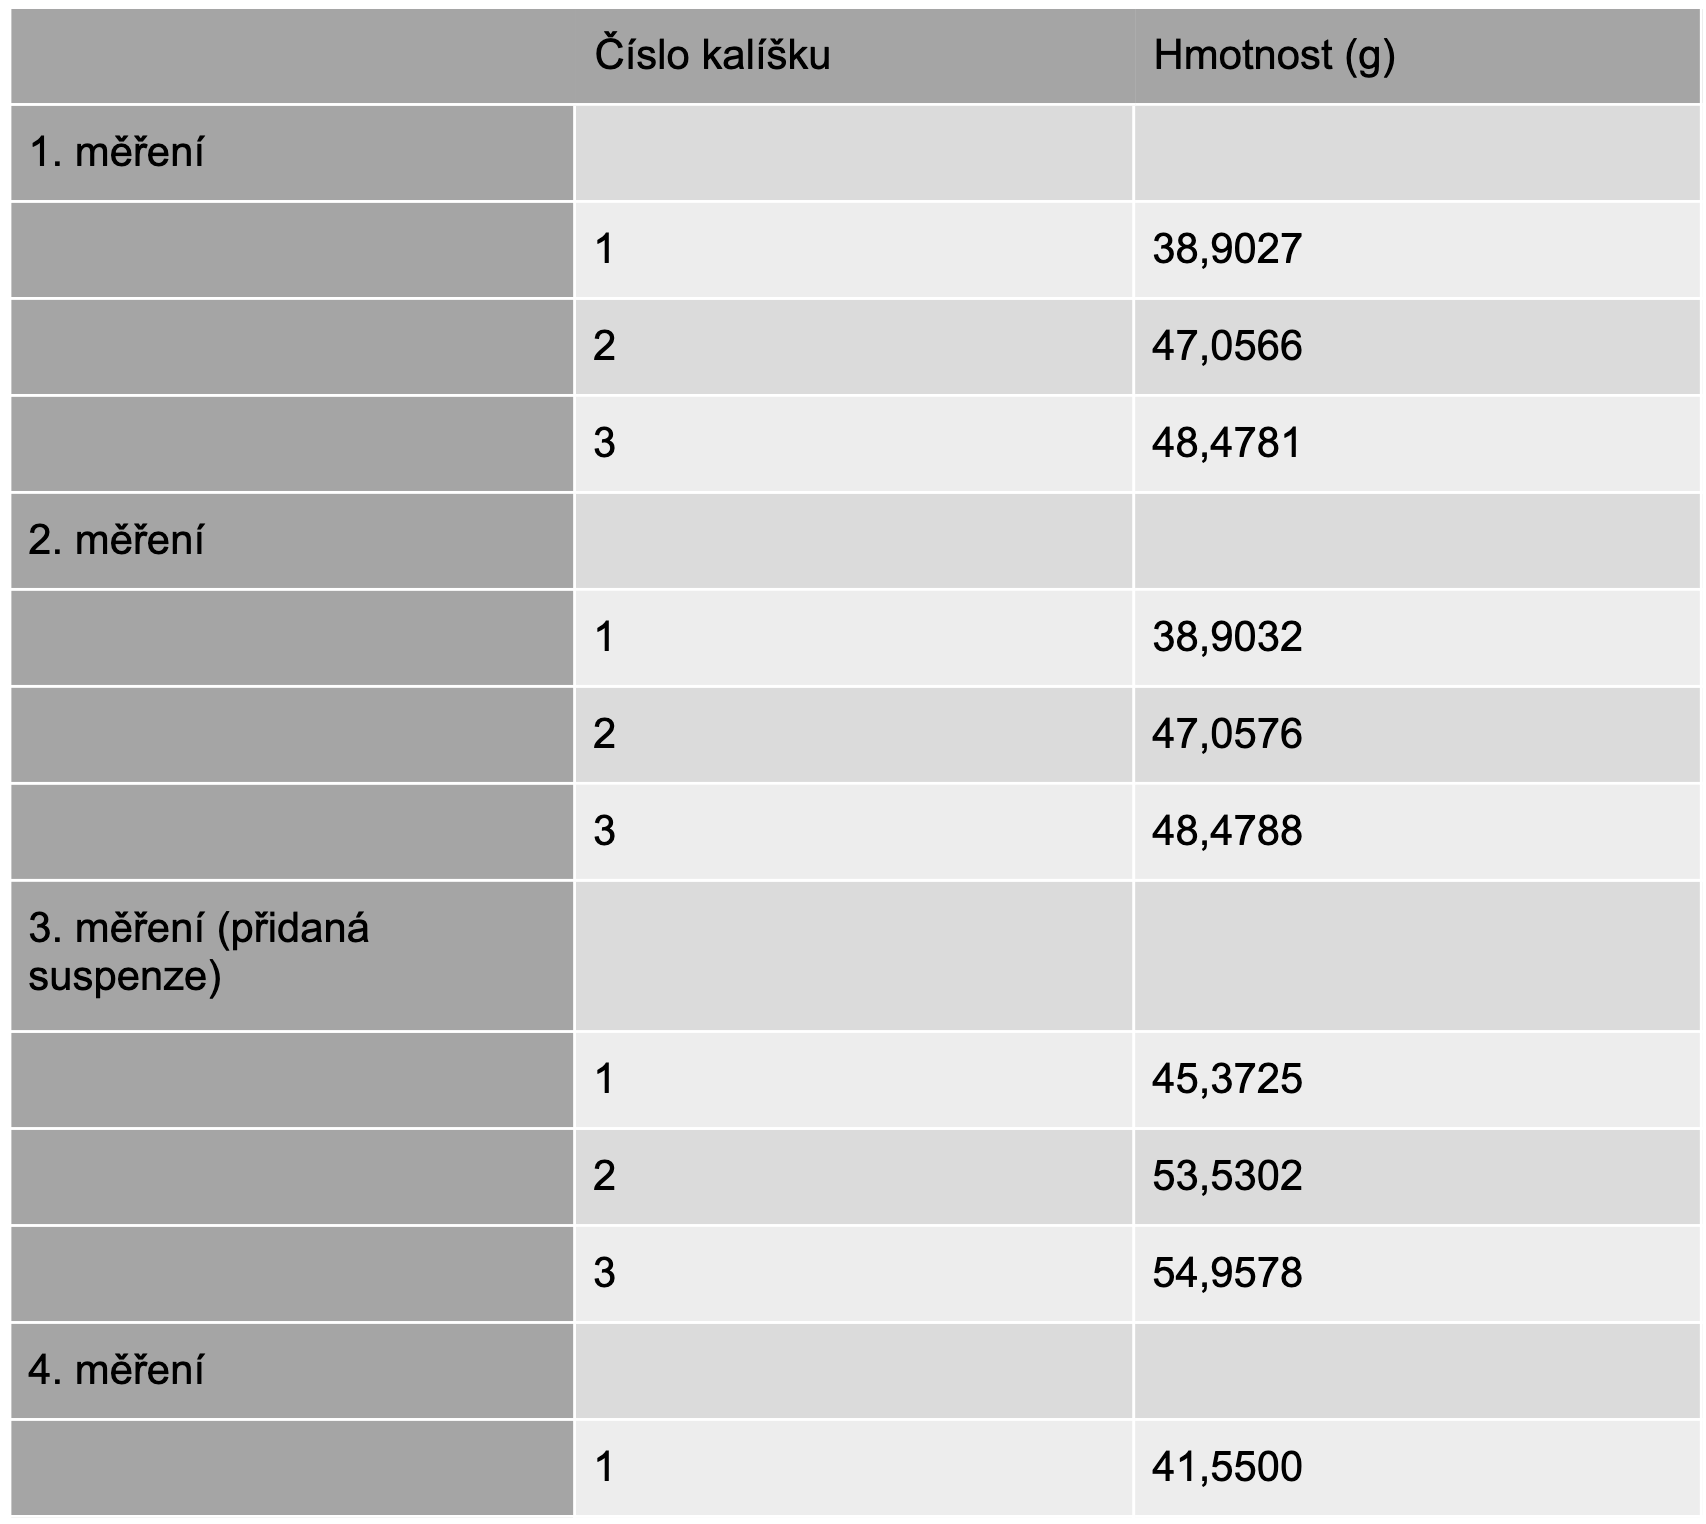
\includegraphics[width=6.8in]{tab_uloha10_1.png}
\end{figure}

\begin{figure}[H]
    \centering
    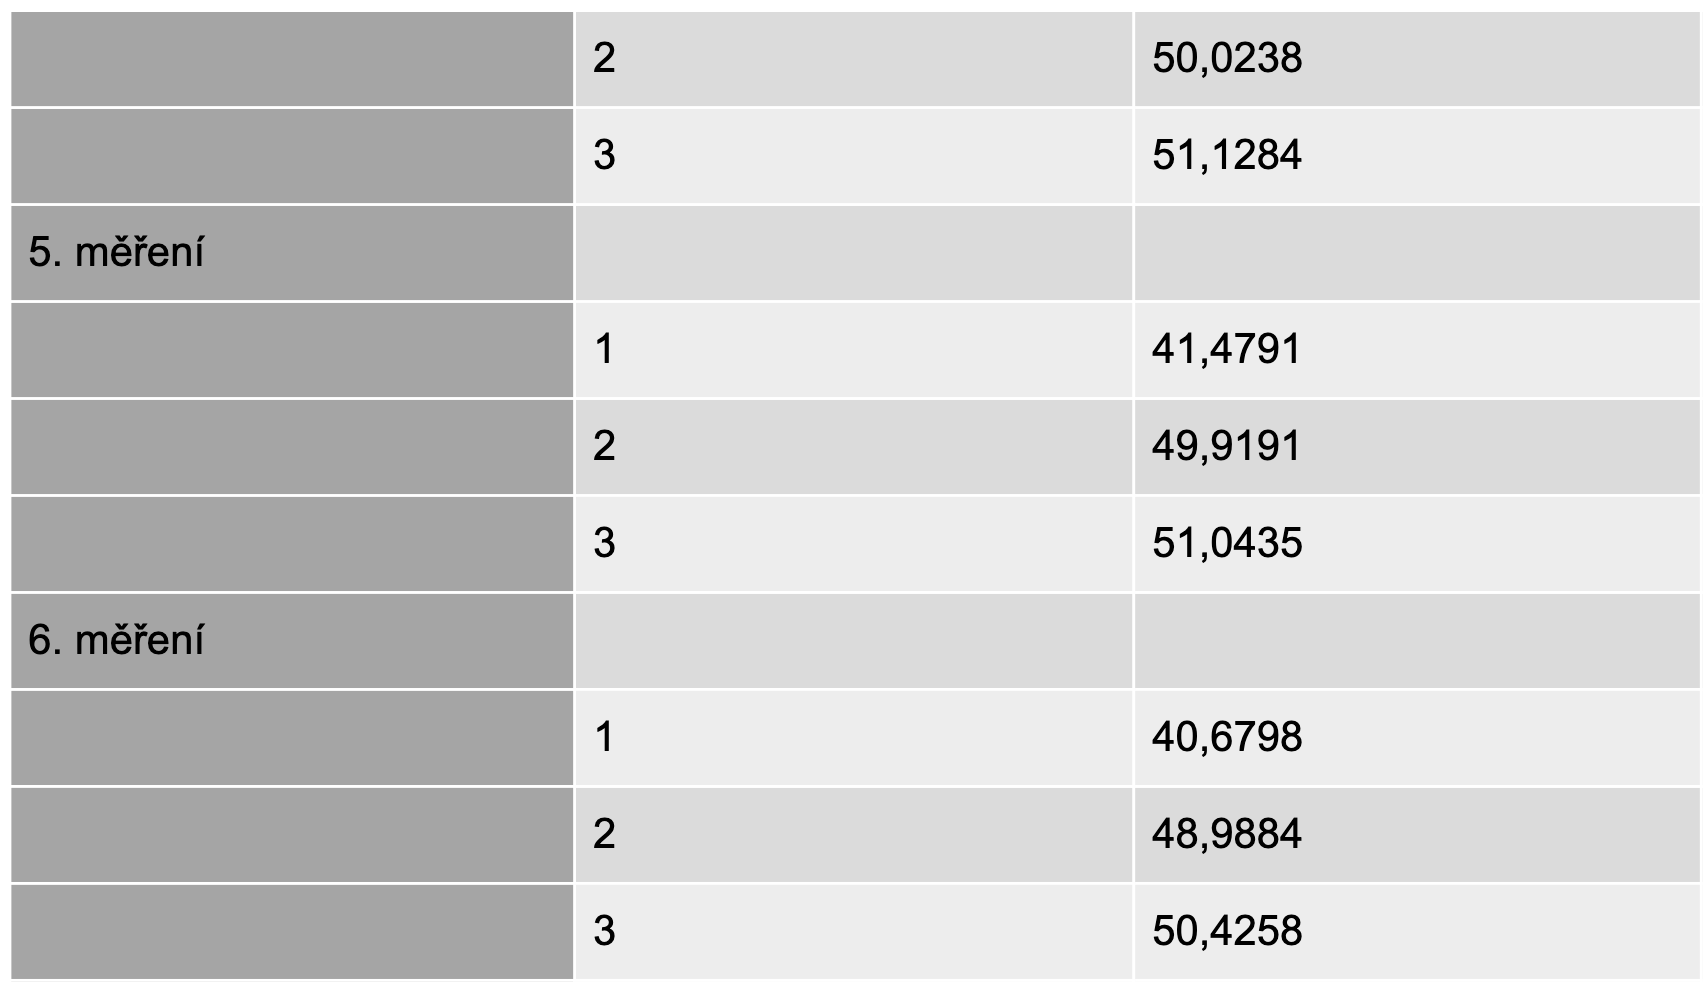
\includegraphics[width=6.8in]{tab_uloha10_2.png}
    \caption*{Tab. 1: žíhání do konstantní hmotnosti při stanovení rozpustnosti a identifikace roztoku
    }
\end{figure}

\begin{figure}[H]
    \centering
    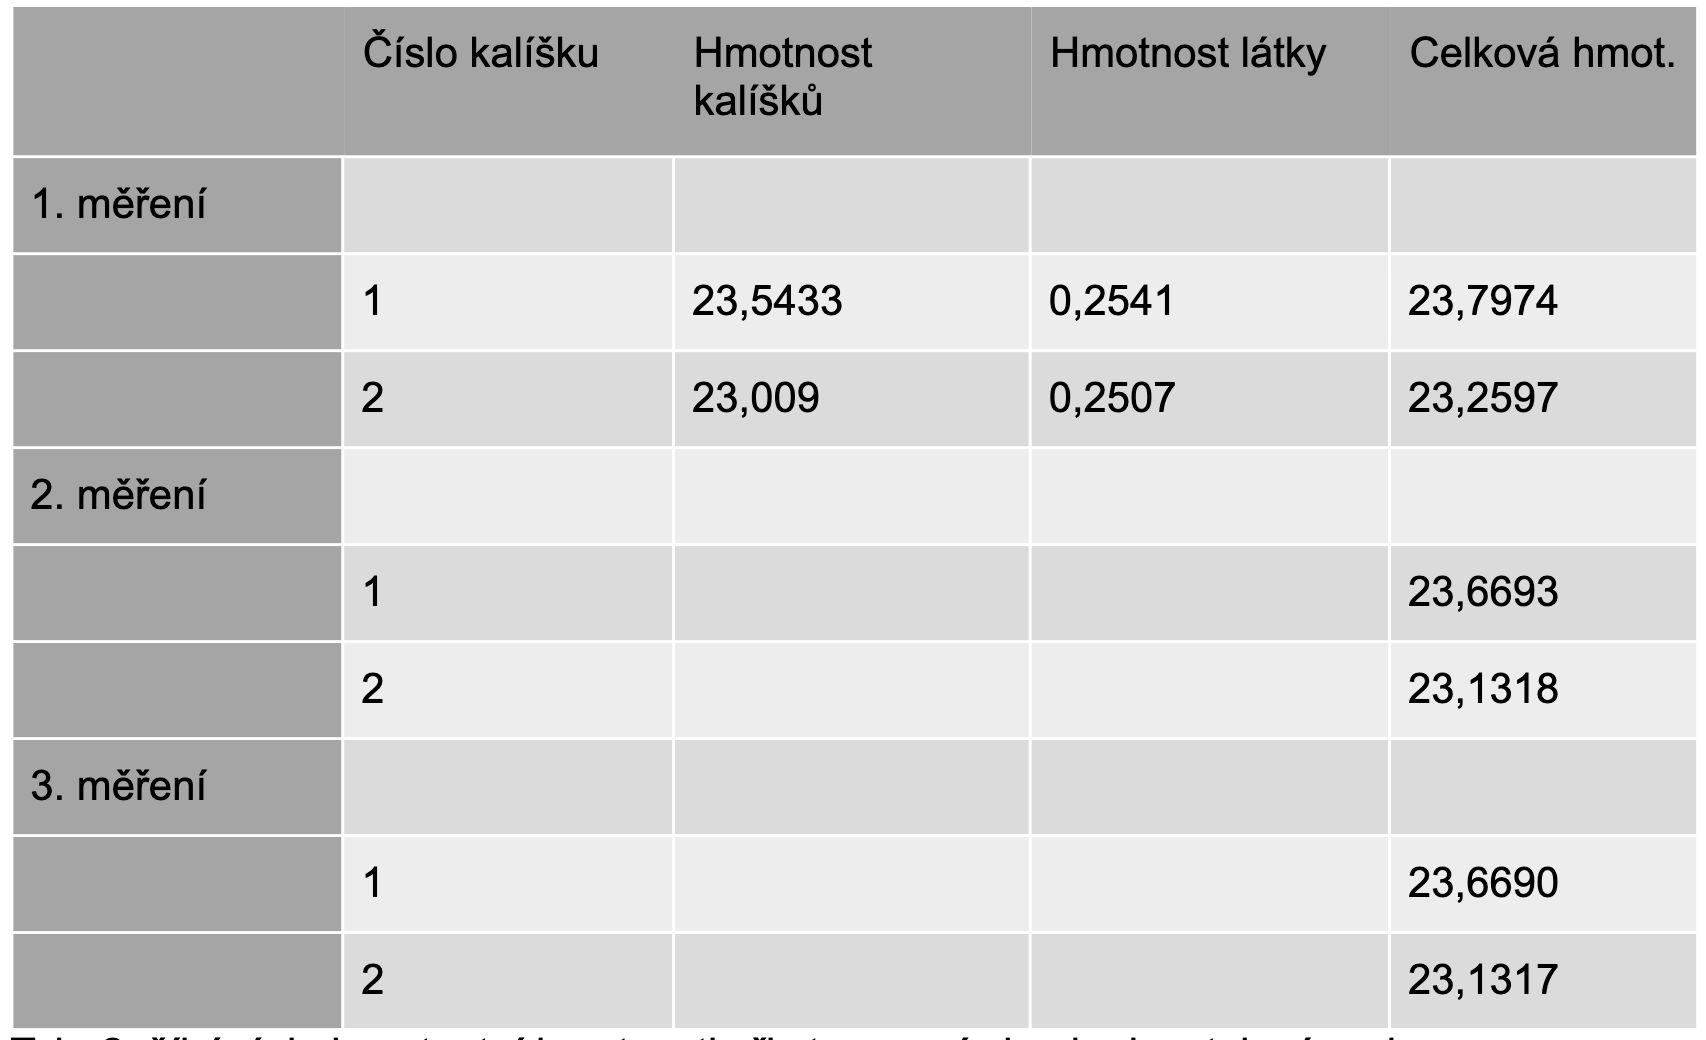
\includegraphics[width=6.8in]{tab_uloha10_3.png}
    \caption*{Tab. 2: žíhání do konstantní hmotnosti při stanovení obsahu krystalové vody}
\end{figure}

\section*{Výpočty}
\subsection*{Stanovení rozpustnosti a identifikace vzorku}
\begin{align*}
    m_{1(vzorek)}&=6,4693\: g\\
    m_{2(vzorek)}&= 6,479\: g\\
    m_{3(vzorek)}&= 6,479\: g
\end{align*}
\newpage
\begin{align*}
    m_{1(vytezek)}&= 1,7766\: g\\
    m_{2(vytezek)}&= 1,9308\: g\\
    m_{3(vytezek)}&= 1,947\: g
\end{align*}

\begin{align*}
    m_{1(odparenevody)}&= 4,6927\: g\\
    m_{2(odparenevody)}&= 4,5418\: g\\
    m_{3(odparenevody)}&= 4,532\: g
\end{align*}


\begin{align*}
    \rho_1 = 1,2939\: g\cdot cm^{-3}\\
    \rho_2 = 1,2945\: g\cdot cm^{-3}\\
    \rho_3 = 1,2958\: g\cdot cm^{-3}\\
    \rho_{prumer} = 1,2947\: g\cdot cm^{-3}
\end{align*}

\subsection*{Rozpustnost}
\subsubsection*{gramy rozpuštěné látky/100 ml roztoku}
\begin{center}
$1,8848 \:g$……………$5 \: ml$\\
$x\: g$……………$100 \: ml$
\end{center}

\begin{align*}
    x &= \frac{100}{5} \cdot 1.8848\\
    x &= 37,696 \: g\cdot 100ml^{-1}\: roztoku
\end{align*}

\subsubsection*{gramy rozpuštěné látky/100 g roztoku}
\begin{center}
$1,8848 \:g$……………$6,4758 \:g$\\
$y \:g$……………$100 \:g$
\end{center}

\begin{align*}
    y = \frac{100}{6,4758} \cdot 1,8848\\
    y = 29,1052\: g\cdot 100g^{-1} \: roztoku
\end{align*}

\subsubsection*{gramy rozpuštěné látky/100 g vody}
\begin{center}
$1,8848\: g$……………$4,5888\: g$\\
$z\: g$……………$100\: g$
\end{center}

\begin{align*}
    z = \frac{100}{4,5888} \cdot 1,8848\\
    z = 41,0739 \: g\cdot 100g^{-1} vody
\end{align*}

\subsection*{Molární koncentrace}
$V= 0,005 \: dm^3$\\
$c=\frac{n}{V}$

\begin{align*}
    n&= \frac{m_{vytezek}}{M_{r(MgSO_4)}}\\
    n&= 0,016 \:mol\\
    \to &c=3,2 \: mol \cdot dm^{-3}
\end{align*}

\subsection*{Molalita}
\begin{align*}
    c_m = \frac{n}{m_{rozpoistedlo}}\\
    c_m = 3,5 mol \cdot kg^{-1}
\end{align*}

\subsection*{Stanovený počet molekul krystalové vody}
\begin{align*}
    m_{H_2O} &= 0,1282\: g\\
    \to m &= \frac{m_{H_20}}{M_{r(H_2O)}}\\
    n &= 0,0071\: mol \\
    \to N &= 4,28 \cdot 10^{21}
\end{align*}

\begin{align*}
    m_{MgSO_4} &= 0,124\: g \\
    Mr_{MgSO_4} &= 120,36 \: g\cdot mol^{-1}\\
    \to n_{MgSO_4} &= \frac{m_{MgSO_4}}{Mr_{MgSO_4}}\\
    n_{MgSO_4} &= 0,00103 \:mol\\
    \to N_{MgSO_4} &= 6,21 \cdot 10^{20}\\
    \to \frac{N_{H_2O}}{N_{MgSO_4}} &= 7,13 \Rightarrow  \text{heptahydrát}
\end{align*}

\section*{Závěr}
Na základě rozpustnosti byl neznámý vzorek č. 105 identifikován jako síran hořečnatý. Byla spočítána hustota
$\rho_{prumer}=1,2947 \: g \cdot cm^{-3}$, molární koncentrace $c=3,2 mol \cdot dm^{-3}$
a molalita $c_m3,5 \: mol \cdot kg^{-1}$. Rozpustnost síranu hořečnatého je
$x=37,696 \: g \cdot ml^{-1}$ roztoku, $29,1052\: g \cdot 100 g^{-1}$ roztoku
a $41,0739\: g \cdot 100g^{-1}$.












\end{document}